\documentclass[ms]{byuprop}
% Options for this class include the following (* indicates default):
%
%   10pt -- 10 point font size
%   11pt -- 11 point font size
%   12pt (*) -- 12 point font size
%
%   ms -- produce a thesis proposal (off)
%   areaexam -- produce a research area overview (off)
%   phd -- produce a dissertation proposal (off)
%   
%   layout -- show layout lines on the pages, helps with overfull boxes (off)
%   grid -- show a half-inch grid on every page, helps with printing (off)


% This command fixes my particular printer, which starts 0.03 inches too low,
% shifting the whole page down by that amount.  This shifts the document
% content up so that it comes out right when printed.
%
% Discovering this sort of behavior is best done by specifying the ``grid''
% option in the class parameters above.  It prints a 1/2 inch grid on every
% page.  You can then use a ruler to determine exactly what the printer is
% doing.
%
% Uncomment to shift content up (accounting for printer problems)
%\setlength{\voffset}{-.03in}

% Here we set things up for invisible hyperlinks in the document.  This makes
% the electronic version clickable without changing the way that the document
% prints.  It's useful, but optional.
\usepackage[
    ps2pdf,
    bookmarks=true,
    breaklinks=true,
    raiselinks=true,
    pdfborder={0 0 0},
    colorlinks=false,
    ]{hyperref}

% Rewrite the itemize, description, and enumerate environments to have more
% reasonable spacing:
\newcommand{\ItemSep}{\itemsep 0pt}
\let\oldenum=\enumerate
\renewcommand{\enumerate}{\oldenum \ItemSep}
\let\olditem=\itemize
\renewcommand{\itemize}{\olditem \ItemSep}
\let\olddesc=\description
\renewcommand{\description}{\olddesc \ItemSep}

% Get a little less fussy about word spacing on a line.  Sometimes produces
% ugly results, so keep your eyes peeled.
\sloppy

% Important settings for the byuprop class. %
%%%%%%%%%%%%%%%%%%%%%%%%%%%%%%%%%%%%%%%%%%%%%

% Because I use these things in more than one place, I created new commands for
% them.  I did not use \providecommand because I absolutely want LaTeX to error
% out if these already exist.
\newcommand{\Title}{A Speculative Approach to Parallelization in Particle Swarm
Optimization}
\newcommand{\Author}{Matthew Gardner}
\newcommand{\SubmissionMonth}{February}
\newcommand{\SubmissionYear}{2011}

% Take these from the commands defined above
\title{\Title}
\author{\Author}
\monthsubmitted{\SubmissionMonth}
\yearsubmitted{\SubmissionYear}

% Committee members
\committeechair{Kevin Seppi}
\committeemembera{Dan Ventura}
\committeememberb{David Embley}
%\committeememberc{}
%\committeememberd{}

% Department graduate coordinator
\graduatecoordinator{Kent Seamons}

%%%%%%%%%%%%%%%%%%%%%%%%%%%%%%%%%%%%%%%%%%%%%

% Set up the internal PDF information so that it becomes part of the document
% metadata.  The pdfinfo command will display this. Be sure to set the document
% type and add your own keywords.
\hypersetup{%
    pdftitle=\Title,%
    pdfauthor=\Author,%
    pdfsubject={Masters thesis proposal, BYU CS Department: %
                Submitted \SubmissionMonth~\SubmissionYear, Created \today},%
    pdfkeywords={parallel algorithms, optimization methods, particle swarm %
				optimization, speculative decomposition},%
}

% These packages allow the bibliography to be sorted alphabetically and allow references to more than one paper to be sorted and compressed (i.e. instead of [5,2,4,6] you get [2,4-6])
\usepackage{url}
\usepackage[numbers,sort&compress]{natbib}
\bibliographystyle{annotnat}
\usepackage{hypernat}
% Note, use \citet to name the authors (text mode) and \citep to do just give
% the number (parenthetical mode).  Also, \citep* will give all of the authors
% rather than an abbreviated list.

% Additional packages required for your specific thesis go here. I've left some I use as examples.
\usepackage{graphicx}
\usepackage{psfrag}
%\usepackage{pdfsync}
\usepackage{amsmath}

% Better references, I think
\newcommand{\secref}[1]{Section~\ref{sec:#1}}
\newcommand{\figref}[1]{Figure~\ref{fig:#1}}
\newcommand{\algref}[1]{Algorithm~\ref{alg:#1}}

%% PSO Stuff
\DeclareMathOperator*{\argmin}{arg\;min}
\DeclareMathOperator*{\argmax}{arg\;max}
\DeclareMathOperator*{\arginf}{arg\;inf}
\DeclareMathOperator*{\argsup}{arg\;sup}
\providecommand{\pers}{\ensuremath{P}}
\providecommand{\neigh}{\ensuremath{N}}
\providecommand{\leftind}{\ensuremath{L}}
\providecommand{\rightind}{\ensuremath{R}}
\providecommand{\nURand}{\ensuremath{U^\neigh}}
\providecommand{\pURand}{\ensuremath{U^\pers}}
\providecommand{\ppos}{\ensuremath{\Vec{x}}}
\providecommand{\fppos}{\ensuremath{\Vec{fx}}}
\providecommand{\pvel}{\ensuremath{\Vec{v}}}
\providecommand{\nbest}{\ensuremath{\Vec{b}^\neigh}}
\providecommand{\fnbest}{\ensuremath{\Vec{fb}^\neigh}}
\providecommand{\pbest}{\ensuremath{\Vec{b}^\pers}}
\providecommand{\fpbest}{\ensuremath{\Vec{fb}^\pers}}
\providecommand{\constriction}{\ensuremath{\chi}}
\providecommand{\ncoeff}{\ensuremath{\phi^\neigh}}
\providecommand{\pcoeff}{\ensuremath{\phi^\pers}}
\providecommand{\obs}{\ensuremath{\Vec{\xi}}}
\providecommand{\ofunc}{\ensuremath{f}}
\providecommand{\swarm}{\ensuremath{swarm}}

%SpecExPSO Stuff
\providecommand{\indic}{\ensuremath{I}}
\providecommand{\specvel}{\ensuremath{\vec{V}}}
\providecommand{\specpos}{\ensuremath{\vec{X}}}
\providecommand{\leftn}{\ensuremath{\Vec{x}^\leftind}}
\providecommand{\rightn}{\ensuremath{\Vec{x}^\rightind}}
\providecommand{\caseset}{\ensuremath{\mathcal{C}}}
\providecommand{\casegen}{\ensuremath{c}}
\providecommand{\casedef}{\ensuremath{(\pbest,\nbest)}}
\providecommand{\casexn}{\ensuremath{(S,-)}}
\providecommand{\casexx}{\ensuremath{(S,S)}}
\providecommand{\casexl}{\ensuremath{(S,\leftind)}}
\providecommand{\casexr}{\ensuremath{(S,\rightind)}}
\providecommand{\casepn}{\ensuremath{(-,-)}}
\providecommand{\casepl}{\ensuremath{(-,\leftind)}}
\providecommand{\casepr}{\ensuremath{(-,\rightind)}}
\providecommand{\casepN}{\ensuremath{(-,N)}}
\providecommand{\casexN}{\ensuremath{(S,N)}}
\providecommand{\noeval}[1]{\ensuremath{#1^{-e}}}
\providecommand{\nonbest}[1]{\ensuremath{#1^{-n}}}
\providecommand{\p}{\ensuremath{p}}
\providecommand{\pset}{\ensuremath{\mathbf{p}}}
\providecommand{\s}{\ensuremath{s}}
\providecommand{\sset}{\ensuremath{\mathbf{s}}}
\providecommand{\nsset}{\ensuremath{\mathbf{ns}}}
\providecommand{\n}{\ensuremath{n}}
\providecommand{\nset}{\ensuremath{\mathbf{n}}}
\providecommand{\nnset}{\ensuremath{\mathbf{nn}}}

%Other math
\providecommand{\prob}{\ensuremath{\mathrm{Pr}}}


\begin{document}

% Produce the preamble
\maketitle


%%%%%%%%%%%%%%%%%%%%%%%%%%%%%%%%%%%%%%%%%%%%%%%%%%%%%%%%%%%%%%%%%%%%%%%%%%%%%%

\section{Abstract}
% 1 to 2 paragraphs

Particle swarm optimization (PSO) is an evolutionary algorithm that has proven
effective at solving complicated optimization problems.  Since its inception,
however, PSO has been run primarily in serial on a single machine.  With the
world's computing resources increasingly coming from large clusters of
processors, the parallelization of the algorithm is important to its continued
relevance.  PSO has previously been parallelized primarily by distributing the
computation corresponding to particles across multiple processors.  In these
approaches, additional processors can only add more particles to the swarm.
However, in many cases this is not efficient when scaled to very large swarm
sizes (on very large clusters).  Current methods cannot answer well the
question, ``What do you do with 1000 processors when 50 or 100 particles is the
most efficient swarm size?''  In this project we attempt to answer that
question with a speculative approach to the parallelization of PSO motivated by
speculative execution in modern computer hardware.

In our approach, we refactor PSO such that the computation needed for iteration
$t+1$ can be done in parallel with the computation needed for iteration $t$.
Thus we can perform two iterations of PSO at once.  Even with some amount of
wasted computation, we show that this approach to parallelization in PSO often
outperforms the na\"ive parallelization of simply adding particles to the
swarm.  Our methods produce results that are exactly equivalent to PSO; this is
not a new algorithm or variant, only a new method of parallelization.

However, given this new parallelization model we can relax the requirement of
exactly reproducing PSO in an attempt to produce better results.  We present
several such relaxations, including keeping the best speculative position
evaluated instead of the one corresponding to PSO, and speculating several
iterations ahead instead of just one.  We show that these methods dramatically
improve the performance of parallel PSO in many cases.

%%%%%%%%%%%%%%%%%%%%%%%%%%%%%%%%%%%%%%%%%%%%%%%%%%%%%%%%%%%%%%%%%%%%%%%%%%%%%%

\section{Introduction}
% 1 to 4 pages
\label{sec:intro}

Particle swarm optimization (PSO) has been found to be a highly robust and
effective algorithm for solving many types of optimization
problems~\citep{poli-2008-pso-applications}.  For much of the algorithm's
history, PSO was run serially on a single machine.  However, the world's
computing power is increasingly coming from large clusters of processors.  In
order to efficiently utilize these resources for computationally intensive
problems, PSO needs to run in parallel.

Within the last few years, researchers have begun to recognize the need to
develop parallel implementations of PSO, publishing many papers on the subject.
The methods they have used include various synchronous algorithms
\citep{chu-2006-intelligent-parallel-pso,jin-2005-pso-antenna-designs,%
parsopoulos-2004-parallel-vector-evaluated-pso,%
schutte-2004-parallel-global-optimization-with-pso} and asynchronous algorithms
\citep{mostaghim-2006-multi-objective-pso-on-grids,%
venter-2005-parallel-pso-asynchronous-evaluations}.  Parallelizing the
evaluation of the objective function can also be done in some cases, though
that is not an adaption of the PSO algorithm itself and thus is not the focus
of this project.

These previous parallel techniques distribute the computation needed by the
particles in the swarm over the available processors.  If more processors are
available, these techniques increase the number of particles in the swarm,
either by adding individual particles or by adding entire new sub-swarms.  In
almost all cases, adding additional particles produces better results in the
same amount of time~\citep{mcnabb-2009-large-particle-swarms}.  In
\figref{iters-sphere} we see an example of this on the well-known benchmark
function Sphere (20 dimensions, reporting the average of twenty runs).  In
terms of the number of iterations performed (which is equivalent to wall-clock
time if all particles are evaluated in parallel), every time the swarm size
increases, the performance improves.

\begin{figure}
  \centering
  \includegraphics[width=.4\columnwidth]{iters_sphere}
  \caption{Function Sphere with various swarm sizes, comparing performance with
  the number of iterations of the algorithm performed.}
  \label{fig:iters-sphere}
\end{figure}

However, it can be seen from the graph that once the swarm is sufficiently
large, doubling the swarm size produces only incremental benefit; performance
improves, but not by very much.  The reason for this is that there comes a
point of diminishing returns with respect to adding particles.  In
\figref{evals-sphere} we show the value obtained after 50,000 function
evaluations (not iterations) as a function of swarm size, again for the
function Sphere.  Increasing the swarm size from 5 to 10 has a significant
effect on the value obtained.  However, increasing the swarm size from 16 to 30
makes the algorithm less efficient; that is, it reduces the progress the
algorithm makes per evaluation.  Other functions show similar trends, though
often the optimal swarm size is slightly larger.  For this reason, previous
work has recommended the use of a swarm size of 50 for
PSO~\citep{bratton-2007-defining-a-standard-for-pso}.  Thus, in at least some
cases, adding particles indefinitely will not yield an efficient
implementation. 

\begin{figure}
  \centering
  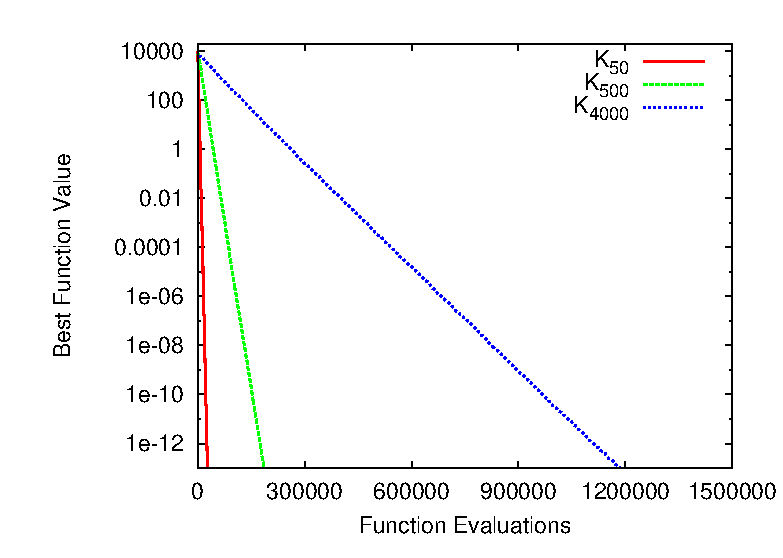
\includegraphics[width=.4\columnwidth]{evals_sphere}
  \caption{Function Sphere with various swarm sizes, comparing performance with
  the number of function evaluations performed.  Error bars show median and
  10th and 90th percentiles.}
  \label{fig:evals-sphere}
\end{figure}

In this project we will consider PSO parallelization strategies for clusters of
hundreds or thousands of processors and functions for which a single evaluation
will take at least tens of seconds, but probably minutes or perhaps hours.  Our
purpose is to explore the question of what to do with a thousand processors
when 50 or 100 particles is the most efficient swarm size, and simply adding
particles results in only incremental improvement.  In our work we assume that
the researcher has some fixed number of processors that should be fully
utilized throughout the optimization process.

In this project we will show that the results of standard PSO can be reproduced
\emph{exactly}, two iterations at a time, using a speculative approach adapted
from speculative execution. We prove that the standard PSO equation can be
factored such that a set of speculative positions can be found which will
always include the position computed in the next iteration.  By computing the
value of the objective function for each of the speculative positions at the
same time the algorithm evaluates the objective function for the current
position, it is possible to know the objective function values for both the
current and the next iteration at the same time.  We will demonstrate this
principle by implementation and show that it produces exactly the same results
as standard PSO, but two iterations at a time.  The resulting implementation
should run efficiently on large clusters where the number of processors is much
larger than a typical or reasonable number of particles, producing better
results in less ``wall-clock'' time.

It is important to note here that this is not a variant of PSO.  We simply
propose a new way to think about the parallelization of PSO that we show
performs better in many cases than previous parallelizations.

Furthermore, we show that if we relax the requirements of the algorithm, no
longer demanding that it strictly reproduce the exact behavior of standard PSO,
we can introduce new speculative techniques that often out-perform na\"ive
parallelizations of PSO.  These relaxations make better use of the information
obtained from the extra exploration made by the speculative function
evaluations.  We also explore the idea that, like branch prediction in
processors, we need not speculatively evaluate \emph{all} possible future
positions, we can accelerate the algorithm even if we are just \emph{likely} to
have guessed right.  By pruning the speculation to just paths that are
statistically likely to reproduce the paths that are equivalent to PSO we can
increase the swarm size without increasing the number of speculative
evaluations.  We also consider several recovery strategies for cases where the
pruned set of speculative evaluations does not contain the evaluation that
standard PSO would have done.  A further improvement we explore is speculating
several iterations ahead instead of just one, which is made possible by pruning
the number of speculative evaluations.

\subsection{Particle Swarm Optimization}
\label{sec:pso}

Particle swarm optimization was proposed in 1995 by James Kennedy and Russell
Eberhart~\citep{kennedy-1995-particle-swarm-optimization}.  The algorithm is
used to intelligently search a multi-dimensional space by mimicking the
swarming and flocking behavior of birds and other animals. It is a social
algorithm that depends on interaction between particles to quickly and
consistently approximate the optimal solution to a given objective function.

The motion of particles through the search space has three components: an
inertial component that gives particles momentum as they move, a cognitive
component where particles remember the best solution they have found and are
attracted back to that place, and a social component by which particles are
attracted to the best solution that any of their neighbors have found.

At each iteration of constricted PSO, the position $\ppos_t$ and velocity
$\pvel_t$ of each particle are updated as follows:
\begin{align}
\label{eq:velupdate}
	\pvel_{t+1} &=
		\constriction \bigl[ \pvel_t
			+ \pcoeff\pURand_{t}\otimes(\pbest_{t} - \ppos_{t}) +
			\ncoeff\nURand_{t}\otimes(\nbest_{t} - \ppos_{t})
		\bigr] \\
\label{eq:posupdate}
	\ppos_{t+1} &= \ppos_{t} + \pvel_{t+1}
\end{align}
where \( \pURand_{t} \) and \( \nURand_{t} \) are vectors of independent random
numbers drawn from a standard uniform distribution, the \( \otimes \) operator
is an element-wise vector multiplication, $\pbest$ (called personal best) is
the best position the current particle has seen, and $\nbest$ (called
neighborhood best) is the best position the neighbors of the current particle
have seen~\citep{bratton-2007-defining-a-standard-for-pso}.  The parameters \(
\ncoeff \), \( \pcoeff \), and \( \constriction \) are given prescribed values
required to ensure convergence (2.05, 2.05, and .73,
respectively)~\citep{clerc-2002-constricted-pso}. 

%%%%%%%%%%%%%%%%%%%%%%%%%%%%%%%%%%%%%%%%%%%%%%%%%%%%%%%%%%%%%%%%%%%%%%%%%%%%%%

\section{Related Work}
\label{sec:related}

There have been several parallel implementations of PSO presented in the
literature.  The improvements described in the literature come in two major
areas: innovations in implementation details and innovations in the use of
topology and swarm size to scale PSO to many processors.

There are many ways to parallelize the basic PSO algorithm.  The most
fundamental decision to make in parallel PSO is which parallel architecture to
use.  Several architectures have been proposed, including Master-Slave, fully
distributed (sometimes called ``diffusion''), and reformulating PSO into
Google's MapReduce framework~\citep{belal-2004-parallel-models-for-pso,
mcnabb-2007-parallel-pso-using-mapreduce}.  A somewhat orthogonal
implementation decision when parallelizing PSO is whether to have synchronous
communication or asynchronous communication.

\subsection{Scaling PSO to many processors}

The other area of research in parallelizing PSO deals not with the
implementation details of architecture and synchronicity, but with what should
be done with the PSO equations when many hundreds or thousands of processors
are available.  The main issues that have been addressed in this space are how
many particles to use for a particular number of processors and what
communication topology should be employed.

The number of particles per processor has typically been decided by how long it
takes to evaluate the function being optimized.  When the function takes longer
than a few seconds to evaluate, previous techniques have assigned the number of
particles in the swarm to be the number of processors available~%
\citep{jin-2005-pso-antenna-designs,mcnabb-2009-large-particle-swarms},
advocating using as many processors as possible to get the best performance.
When the function takes less time to evaluate than the TCP/IP stack used to
send interprocessor communication, parallel implementations assign several or
many particles to a single processor~\citep{chu-2006-intelligent-parallel-pso,
chang-2005-parallel-pso-with-communication-strategies}.  Often the processor
only sends information about the best particle it evaluated to other
processors~\citep{belal-2004-parallel-models-for-pso}.

Another popular method is simply to run PSO independently on each of the
processors available, taking the best result when all of the runs complete.  It
should be noted that this is equivalent to the previously stated method of
assigning many particles to each processor, only with no communication between
processors instead of little communication.  Both of these methods can be
described as changes in the communication topology of the original PSO
algorithm~\citep{mcnabb-2009-large-particle-swarms}.

Thus previous work in parallelizing PSO, apart from implementation details, has
consisted entirely of increasing the swarm size and adapting the topology to be
better suited to parallel computation.

With regard to increasing the swarm size in PSO, some recent work has suggested
that increasing the swarm size throughout the course of the optimization
process provides better results than having a set swarm
size~\citep{hsieh-2009-efficient-population-utilization-for-pso,
montes-de-oca-2010-incremental-social-learning-pso}.  However, these results
focused on serial computation and are based on total number of function
evaluations, which, when running in parallel on expensive functions, is less
important than total number of iterations.  Other work focusing on
parallelization has shown that when extra processors are available they should
be used, as performance increases with swarm size when measuring in terms of
number of iterations~\citep{mcnabb-2009-large-particle-swarms,
jin-2005-pso-antenna-designs}.  If the swarm size were varied throughout the
course of the optimization process, some processors would be sitting idle at
most iterations.

The contribution of our work is in this area of what should be done with the
PSO equations to better utilize a thousand processors when they are available.
In our work we use a synchronous, MapReduce implementation of parallel PSO.
While we use a specific implementation, we describe how speculative evaluation
can be performed in any of the synchronous architectures mentioned in the
previous section.  The adaptation of our methods to asynchronous PSO
parallelization methods should be straightforward, though it is left to future
work.

\section{Thesis Statement}
% 1 to 2 sentences

When many processors are available, a speculative approach to the
parallelization of PSO can yield dramatic improvements in the performance of
the algorithm on expensive functions compared to previous parallelization
techniques.

%%%%%%%%%%%%%%%%%%%%%%%%%%%%%%%%%%%%%%%%%%%%%%%%%%%%%%%%%%%%%%%%%%%%%%%%%%%%%%

\section{Project Description}
% 2 to 5 pages

PSO can be trivially parallelized by assigning each particle's computation to
an individual processor.  But as we have seen in \figref{evals-sphere}, for
some functions, and for large numbers of processors, just adding particles
reaches a point of diminishing returns.  That is, adding processors does not
help the algorithm reach any given level of fitness appreciably faster.
Instead of adding particles we employ a speculative approach that allows us to
perform two iterations at a time.

Our speculative methods require refactoring the PSO equations such that all
possible positions for each particle at iteration $t+1$ can be evaluated in
parallel along with the position of each particle at iteration $t$.  With some
careful bookkeeping, we can then piece together the results of iteration $t+1$
for each particle, thus using extra processors to evaluate two iterations of
the algorithm in the time it takes to evaluate the function once.  A wise
choice of topology limits the necessary speculative evaluations to seven per
particle.

To see the value of this refactoring, suppose that $1000$ processors are
available, and that the evaluation of the objective function takes one hour.
If we only want a swarm of $100$ particles, $900$ of the processors would be
sitting idle for an hour at every iteration, and it would take two hours to run
two iterations.  If instead we perform speculative evaluation, sending each of
the $7$ possible speculative positions of a particle to be computed at the same
time as its current position, we would use $800$ of the $1000$ processors and
perform two iterations in one hour.

In order to do two iterations at once, we must use 8 times as many processors
as there are particles in the swarm.  If these processors were not performing
speculative evaluation, they might instead be used for function evaluations
needed to support a larger swarm.  This raises the question of whether a swarm
of 100 particles doing twice as many iterations outperforms a swarm of 800
particles.  This project will seek to answer that question.

My honors thesis proposed and developed this basic approach to parallelization
in PSO.  This masters thesis will complete the picture of speculative methods
in particle swarm optimization.  First, we present a mathematical proof of
correctness of our methods, given in Section~\ref{sec:proof} as demonstration
that what we propose is in fact mathematically equivalent to standard
parallelization methods in PSO.  Second, we propose pruning the set of possible
speculative evaluations to better use available processors.  We motivate the
pruning by analyzing the statistics of which branches are commonly taken in
PSO, using those statistics to prune all but the most likely branches.
Further, once the idea of pruning is established, we view the set of all
possible speculative evaulations as an infinite tree, not confining ourselves
to speculating only about the next iteration.  We then experiment with
speculating down likely paths three or four iterations ahead, and show that
this by far outperforms simple one-iteration speculative evaluation.  And
lastly, as my honors thesis used only a few experiments on three benchmark
functions, we give a better picture of the performance of speculative
approaches with much more extensive experimentation.

\subsection{Refactoring the PSO Equations}
\label{sec:proof}

To perform two iterations at a time we must first refactor PSO such that the
determination of the value of the objective function is separate from the rest
of the computation.  For simplicity, this discussion will describe the case
where PSO is performing function minimization using the Ring topology.  In this
example, each particle has two neighbors, the ``right neighbor'' and ``left
neighbor,'' whose positions are represented as $\rightn$ and $\leftn$
respectively.  Though we will only describe the case of the Ring topology, this
method can easily be extended to arbitrary topologies (and in fact our
implementation of this algorithm works with arbitrary topologies; we simply
only discuss the Ring case here as that greatly simplifies our notation).

The refactoring hinges on the idea that once the random coefficients
$\pURand_{t}$ and $\nURand_{t}$ are drawn, there are only a few possible new
positions, or updates, for $\nbest$ and $\pbest$.  For the Ring topology there
are 7 possible update cases, identified in Table~\ref{tab:evals}.  We label
each case with an identifier referring to the source of the update: a minus
sign ($-$) represents no update, $L$ represents an update to $\nbest$ coming
from the left neighbor, $R$ represents an update to $\nbest$ coming from the
right neighbor, and $S$ represents an update to either $\pbest$ or $\nbest$
coming from the particle itself.  As an example, $\casexn$ refers to the case
that the particle finds a new personal best, but neither it nor its neighbors
find a position that updated its neighborhood best.  In the equations that
follow, we refer to an unspecified update case as $\casegen$, and to the set of
cases collectively as $\caseset$.

\begin{table}
  \caption{All possible updates for a particle with two neighbors}
  \label{tab:evals}
  \centering
  \begin{tabular}{lcc}
	Identifier&Source of $\pbest$ update&Source of $\nbest$ update\\
	\hline
	\hline
	$\casepn$&No update&No update\\
	\hline
	$\casepl$&No update&Left Neighbor\\
	\hline
	$\casepr$&No update&Right Neighbor\\
	\hline
	$\casexn$&Self&No update\\
	\hline
	$\casexl$&Self&Left Neighbor\\
	\hline
	$\casexr$&Self&Right Neighbor\\
	\hline
	$\casexx$&Self&Self\\
	\hline
  \end{tabular}
\end{table}

In order to incorporate the determination of which case occurs into the
position and velocity update equations, we introduce an indicator function
$\indic_{t+1}^{\casegen}$ for each case $\casegen \in \caseset$.  When
$\casegen$ corresponds to the case actually taken by PSO,
$\indic_{t+1}^{\casegen}$ evaluates to 1; otherwise it evaluates to 0.  We can
then sum over all of the cases, and the indicator function will make all of the
terms drop to zero except for the case that actually occurs.  For example, the
indicator function for the specific case $\casexn$ (which, as is shown in
Table~\ref{tab:evals}, means that the particle's personal best was updated, but
its neighborhood best was not) can be written as follows:

\begin{align}
  \nonumber
	\indic_{t+1}^{\casexn} & (\ofunc ( \ppos_{t} ) ,\ofunc(\leftn_{t}),
	\ofunc(\rightn_{t}) ,\ofunc(\pbest_{t-1}) ,\ofunc(\nbest_{t-1}))= \\
  \label{eq:deficasexn}
	&\begin{cases}
	   1 & \text{if} \ \ofunc(\ppos_{t}) < \ofunc(\pbest_{t-1}) \\
	   &\quad \text{and} \quad \ofunc(\nbest_{t-1}) < \ofunc(\ppos_{t}) \\
	   &\quad \text{and} \quad \ofunc(\nbest_{t-1}) < \ofunc(\leftn_{t}) \\
	   &\quad \text{and} \quad \ofunc(\nbest_{t-1}) < \ofunc(\rightn_{t}) \\
	   0 & \text{otherwise}
	\end{cases}
\end{align}

For each case $\casegen \in \caseset$, there is also a corresponding
velocity update function $\specvel_{t+1}^{\casegen}$.  When the case is
known, the specific values of $\pbest_t$ and $\nbest_t$ may be substituted
directly into~\eqref{eq:velupdate}.  For example, in case $\casexn$,
$\pbest_{t}=\ppos_{t}$, as \pbest was updated by the particle's current
position, and $\nbest_{t}=\nbest_{t-1}$, as $\nbest$ was not updated at
iteration $t$:
\begin{align}
\nonumber
	\specvel_{t+1}^{\casexn} & (\pvel_t, \ppos_{t}, \leftn_{t}, \rightn_{t},
	\pbest_{t-1}, \nbest_{t-1}, \pURand_{t}, \nURand_{t}) \\
\label{eq:defvcasexn}
		&= \constriction \bigl[ \pvel_{t} +
			\pcoeff\pURand_{t}\otimes(\ppos_{t} - \ppos_{t})
			+ \ncoeff\nURand_{t}\otimes(\nbest_{t-1} -
			\ppos_{t}) \bigr]
\end{align}

In the same way we can create notation for the position update function by
substituting into~\eqref{eq:posupdate}.  For compactness, we will drop the
parameters to $\specvel_{t+1}^{\casegen}$ since they can be inferred from the
subscripts.
\begin{align}
\label{eq:defpcasegen}
	\specpos_{t+1}^{\casegen} & (\ppos_{t}, \pvel_{t}, \leftn_{t},
	\rightn_{t} ,\pbest_{t-1} ,\nbest_{t-1}, \pURand_{t}, \nURand_{t})
	= \ppos_{t} + \specvel_{t+1}^{\casegen}
\end{align}

With this notation we can re-write the original PSO velocity
equation~\eqref{eq:velupdate}, introducing our sum over cases with the
indicator functions.  Again, we represent the indicator functions and velocity
functions without the parameters for compactness.  The equation becomes:
\begin{align}
\nonumber
	\pvel_{t+1} &=
		\constriction \bigl[ \pvel_t
			+ \pcoeff\pURand_{t}\otimes(\pbest_{t} - \ppos_{t})
			+ \ncoeff\nURand_{t}\otimes(\nbest_{t} -
			\ppos_{t}) \bigr] \\
\nonumber
	&= \sum_{c \in \caseset} \indic_{t+1}^{c} \ \constriction \bigl[ \pvel_t
			+ \pcoeff\pURand_{t}\otimes(\pbest_{t} - \ppos_{t})
			+ \ncoeff\nURand_{t}\otimes(\nbest_{t} -
			\ppos_{t}) \bigr]  \\
\label{eq:vel2update}
	&= \sum_{c \in \caseset} \ \indic_{t+1}^{c} \ \specvel_{t+1}^{c} 
\end{align}

Similarly, the position update equation~\eqref{eq:posupdate} becomes:
\begin{align}
\label{eq:pos2update}
	\ppos_{t+1} &= \ppos_{t} + \pvel_{t+1}
	= \sum_{c \in \caseset} \ \indic_{t+1}^{c} \ \specpos_{t+1}^{c} 
\end{align}

The value of the objective function at $\ppos_{t+1}$ is given by:
\begin{align}
\label{eq:val2update}
	\ofunc (\ppos_{t+1}) = \sum_{c \in \caseset} \ \indic_{t+1}^{c}
	\ \ofunc(\specpos_{t+1}^{c})
\end{align}

Returning our attention to the computation of $\ppos_{t+1}$ in
\eqref{eq:pos2update} and writing it with the parameters which were omitted
above, we obtain:
\begin{align}
\nonumber
  \ppos_{t+1} = \sum_{c \in \caseset}
	&\indic_{t+1}^{c}(\ofunc ( \ppos_{t} ) ,\ofunc(\leftn_{t}),
	\ofunc(\rightn_{t}) ,\ofunc(\pbest_{t-1}) ,\ofunc(\nbest_{t-1})) \\
\label{eq:val2updatelong}
	& \specpos_{t+1}^{c}(\ppos_{t},\pvel_{t},\leftn_{t},\rightn_{t},
	\pbest_{t-1},\nbest_{t-1},\pURand_{t}, \nURand_{t})
\end{align}

In this form the important point to notice is that there are only $7$ values
(for this Ring topology) in the set $\{\specpos_{t+1}^{\casegen}: \casegen \in
\caseset\}$ and that none of them depend upon $f(\ppos_t)$ or any other
objective function evaluation at iteration $t$.  Note also that while there are
random numbers in the equation, they are assumed fixed once drawn for any
particular particle at a specific iteration.  Thus PSO has been refactored such
that the algorithm can begin computing all $7$ of the objective function
evaluations potentially needed in iteration $t+1$ \emph{before} $f(\ppos_t)$ is
computed.  Once the evaluation of $f(\ppos_{t})$ is completed for all particles
only one of the indicator functions $\indic_{t+1}^{\casegen}$ will be set to 1;
hence only one of the positions $\specpos_{t+1}^\casegen$ will be kept.

Although this speculative approach computes $\ofunc(\specpos_{t+1}^{\casegen})$
for all $\casegen \in \caseset$, even those for which $\indic_{t+1}^{\casegen}
= 0$, these extra computations will be ignored, and might just as well never
have been computed.  We call the set of computations
$\{\ofunc(\specpos_{t+1}^{c}) : \casegen \in \caseset\}$ ``speculative
children'' because only one of them will be needed.

\section{Validation}
% 1/2 to 2 pages

This project is expected to produce an implementation of speculative evaluation
in PSO, including several variations on the speculative evaluations performed.
The project will also show that speculative approaches to parallelization in
PSO result in improved performance over non-speculative approaches.

To show improved performance, we will test our methods against previous
parallelization methods on several benchmark functions.  While benchmark
functions themselves take fractions of a second to evaluate and thus have no
need of the kind of parallelization we explore in this project, they also have
no need of particle swarm optimization at all, as they can be solved
analytically.  Yet they are useful to us and to optimization researchers
generally because they stand as surrogates for the kinds of functions
practitioners are actually interested in, and they allow us to explore the
behavior of optimization algorithms on several different classes of functions
in an easy and standardized way.

We will measure our performance on these benchmark functions in terms of the
best value found at each iteration of the algorithms.  We will also compare the
total number of iterations required by each algorithm to reach some specified
value.  The project will be successful if a statistically significant decrease
in the number of iterations is observed.

For each function, we will use the topology that is generally considered to be
best for optimizing that particular function.  When the Complete topology is
considered best, we will instead use a Random topology that we developed that
mimicks the behavior of Complete while being more suited for parallel
computation~\cite{mcnabb-2009-large-particle-swarms}.  

The functions we will use in our comparisons are these common benchmark
functions: Bohachevsky, Griewank, Rastrigin, Sphere, and Schwefel 2.21.  We
will run each function with 20, 50, and 500 dimensions to test the scalability
of our methods up to higher dimensions.  We will also test our methods on a
more typical ``real-world'' problem, that of training a computationally
intensive machine learning algorithm with a large amount of data.  We will
compare our speculative methods to previous parallelization techniques,
including a naive parallelization of just increasing the swarm size, and a
subswarms implementation that uses several smaller, independent swarms.

\section{Thesis Schedule}
% 1/4 to 1/2 page

\begin{itemize}

\item Completed: Implement speculative evaluation in PSO and several
  improvements on it.

\item March 11, 2011: Finish running experiments and incorporate the results
  into the thesis.
  
\item March 15, 2011: Give final draft of thesis to advisor for review.

\item March 22, 2011: submit thesis to second committee member for review.

\item April 5, 2011: submit thesis to third committee member for review.

\item April 19, 2011: defend thesis.

\end{itemize}


%%%%%%%%%%%%%%%%%%%%%%%%%%%%%%%%%%%%%%%%%%%%%%%%%%%%%%%%%%%%%%%%%%%%%%%%%%%%%%

\renewcommand\bibsection{\section{Annotated Bibliography}}
%\newcommand\bibpreamble{Material to be added between heading and entries.}
% 2 to 5 pages

\bibliography{../../../bib/pso/general/bib,%
../../../bib/pso/parallel/bib,%
../../../bib/pso/topology/bib,%
../../../bib/pso/fips/bib,%
../../../bib/aml/bib,%
../../../bib/parallel/bib,%
../../../bib/nfl/bib%
}


\end{document}
